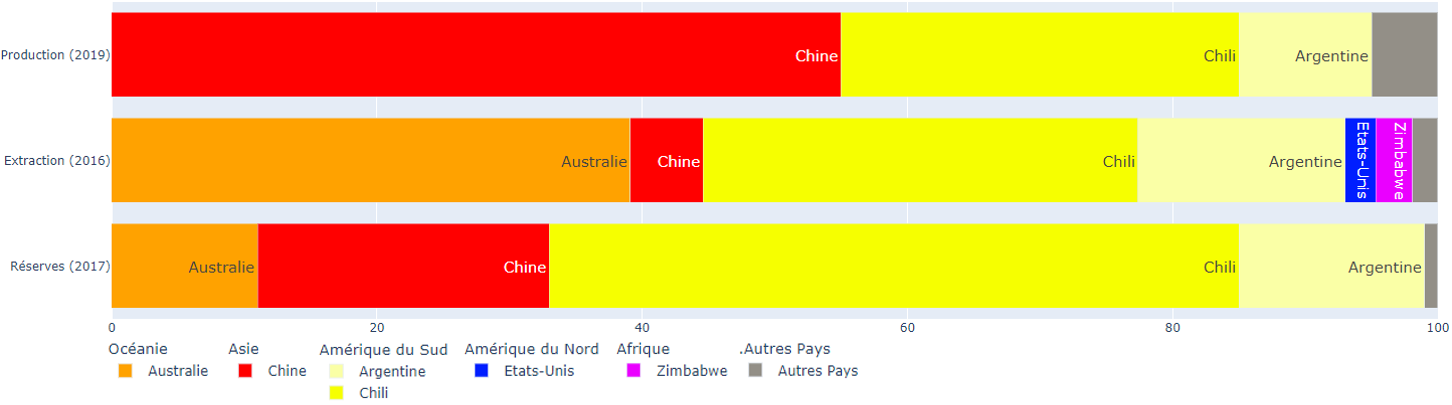
\includegraphics[width=\textwidth]{Illustration métaux/Lithium.png}

\begin{center}
    \textbf{Usage et consommation}
\end{center}
Le lithium est utilisé à 37\% pour la fabrication de batterie et à 30\%
pour la fabrication de verres et céramiques. Dans le domaine énergétique,
le lithium sert exclusivement à la fabrication de batteries.
\begin{center}
    \textbf{Prospective}
\end{center}
\begin{multicols}{2}
    \begin{center}
        \textit{Total lithium demand by sector and scenario}
    \end{center}
    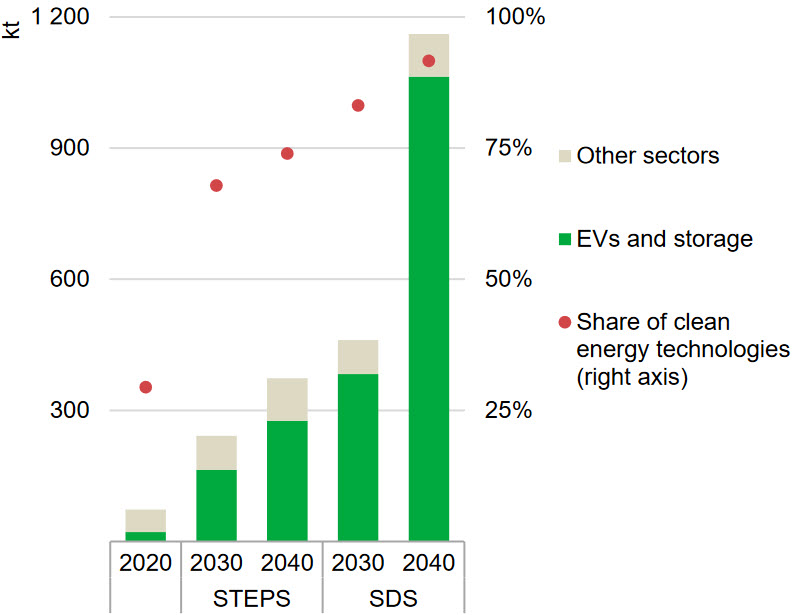
\includegraphics[width=0.45\textwidth]{Illustration métaux/lithium_prospective.jpg}
    \vfill\null
    \columnbreak
    Le lithium est le métal dont la croissance de la demande est prévue
    d'être la plus forte. Cette croissance est causée par la hausse de la
    fabrication de batteries (en majorité pour les véhicules électrique).

    \end{multicols}
\begin{center}
    \textbf{Production et recyclage}
\end{center}
La production minière de lithium a connu un taux de croissance annuel moyen
de 7,8\% entre 2001 et 2016. La production minière dépasse 36 000 kt/an. Moins de 1\% du lithium est recyclé. 
\begin{center}
    \textbf{Substituabilité}
\end{center}
Le lithium dans les batteries peut être substitué en contrepartie de baisse
de performance technologique et de hausse du coût. Les incitations à la substitution
sont faibles en raison de l'évolution technologique en faveur des batteries lithium.
\begin{center}
    \textbf{Prix}
\end{center}
Le prix du lithium est fortement volatile. Il a oscillé entre 6 et 20 US\$/kg entre
2007 et 2018. La valeur de marché de la production annuelle de lithium est de
l'ordre de 2,3 G US\$.
\clearpage
\begin{center}
    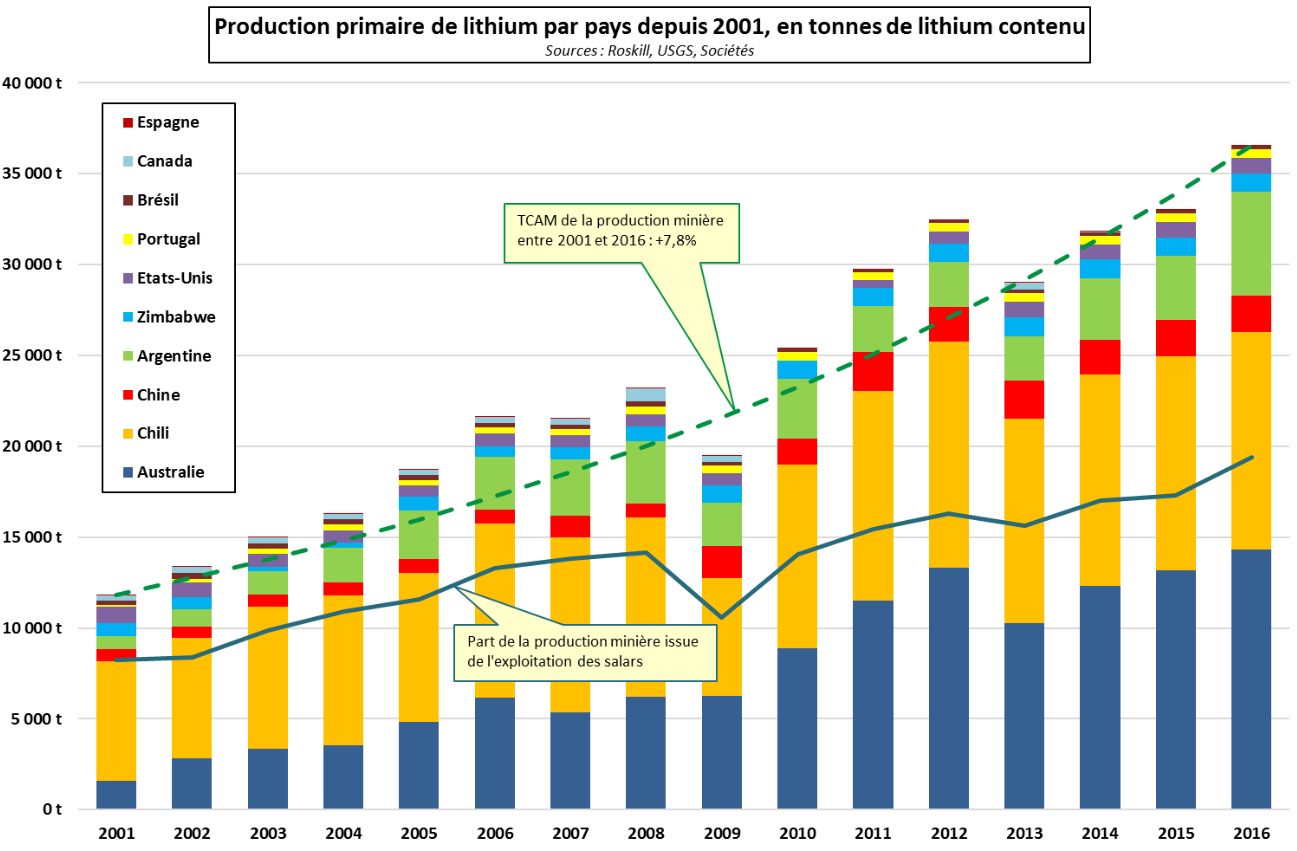
\includegraphics[width=12cm]{Illustration métaux/dynamique_lithium.png}
\end{center}
\begin{center}
    \textbf{Evènements géopolitiques}
\end{center}
Il n'y a pas eu d'évènements géopolitiques notables entre 2000 et 2020.
\begin{multicols}{2}
    \begin{center}
      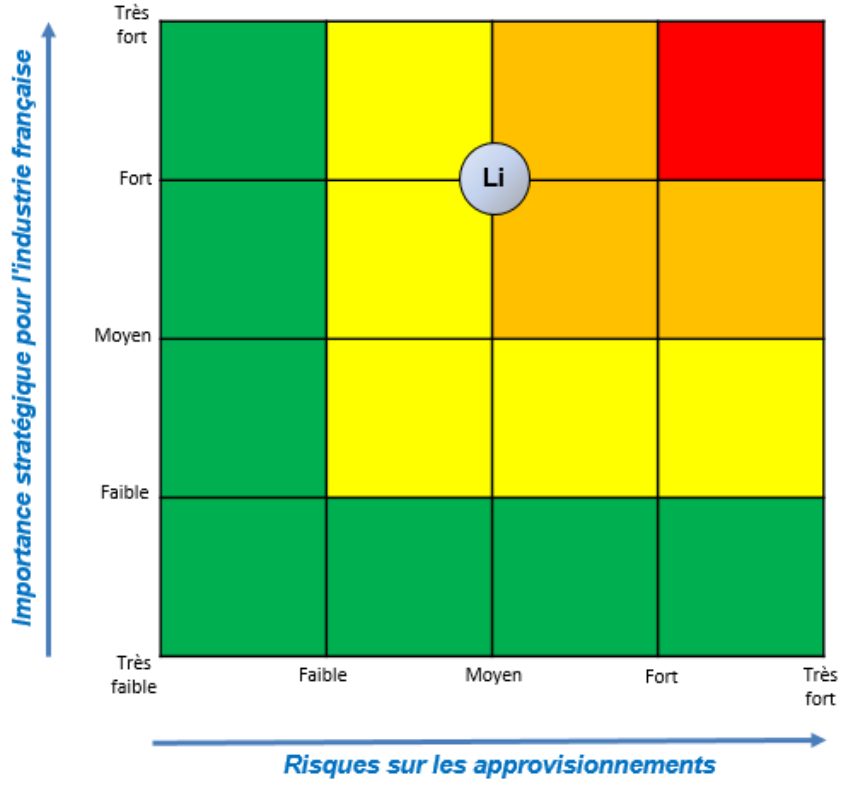
\includegraphics[width=0.35\textwidth]{Illustration métaux/Lithium_criticité.png} 
    \end{center}
    \begin{center}
    \textbf{Criticité en France}
    \end{center}
    Le risque sur les approvisionnements en lithium demeure moyen grâce à une part importante de la production minière située dans des pays de l'OCDE. Le métal reste néanmoins peu substituable et stratégique pour l'électronique et les véhicules électriques.
\end{multicols}
\begin{wrapfigure}{R}{0.65\textwidth}
  \begin{center}
    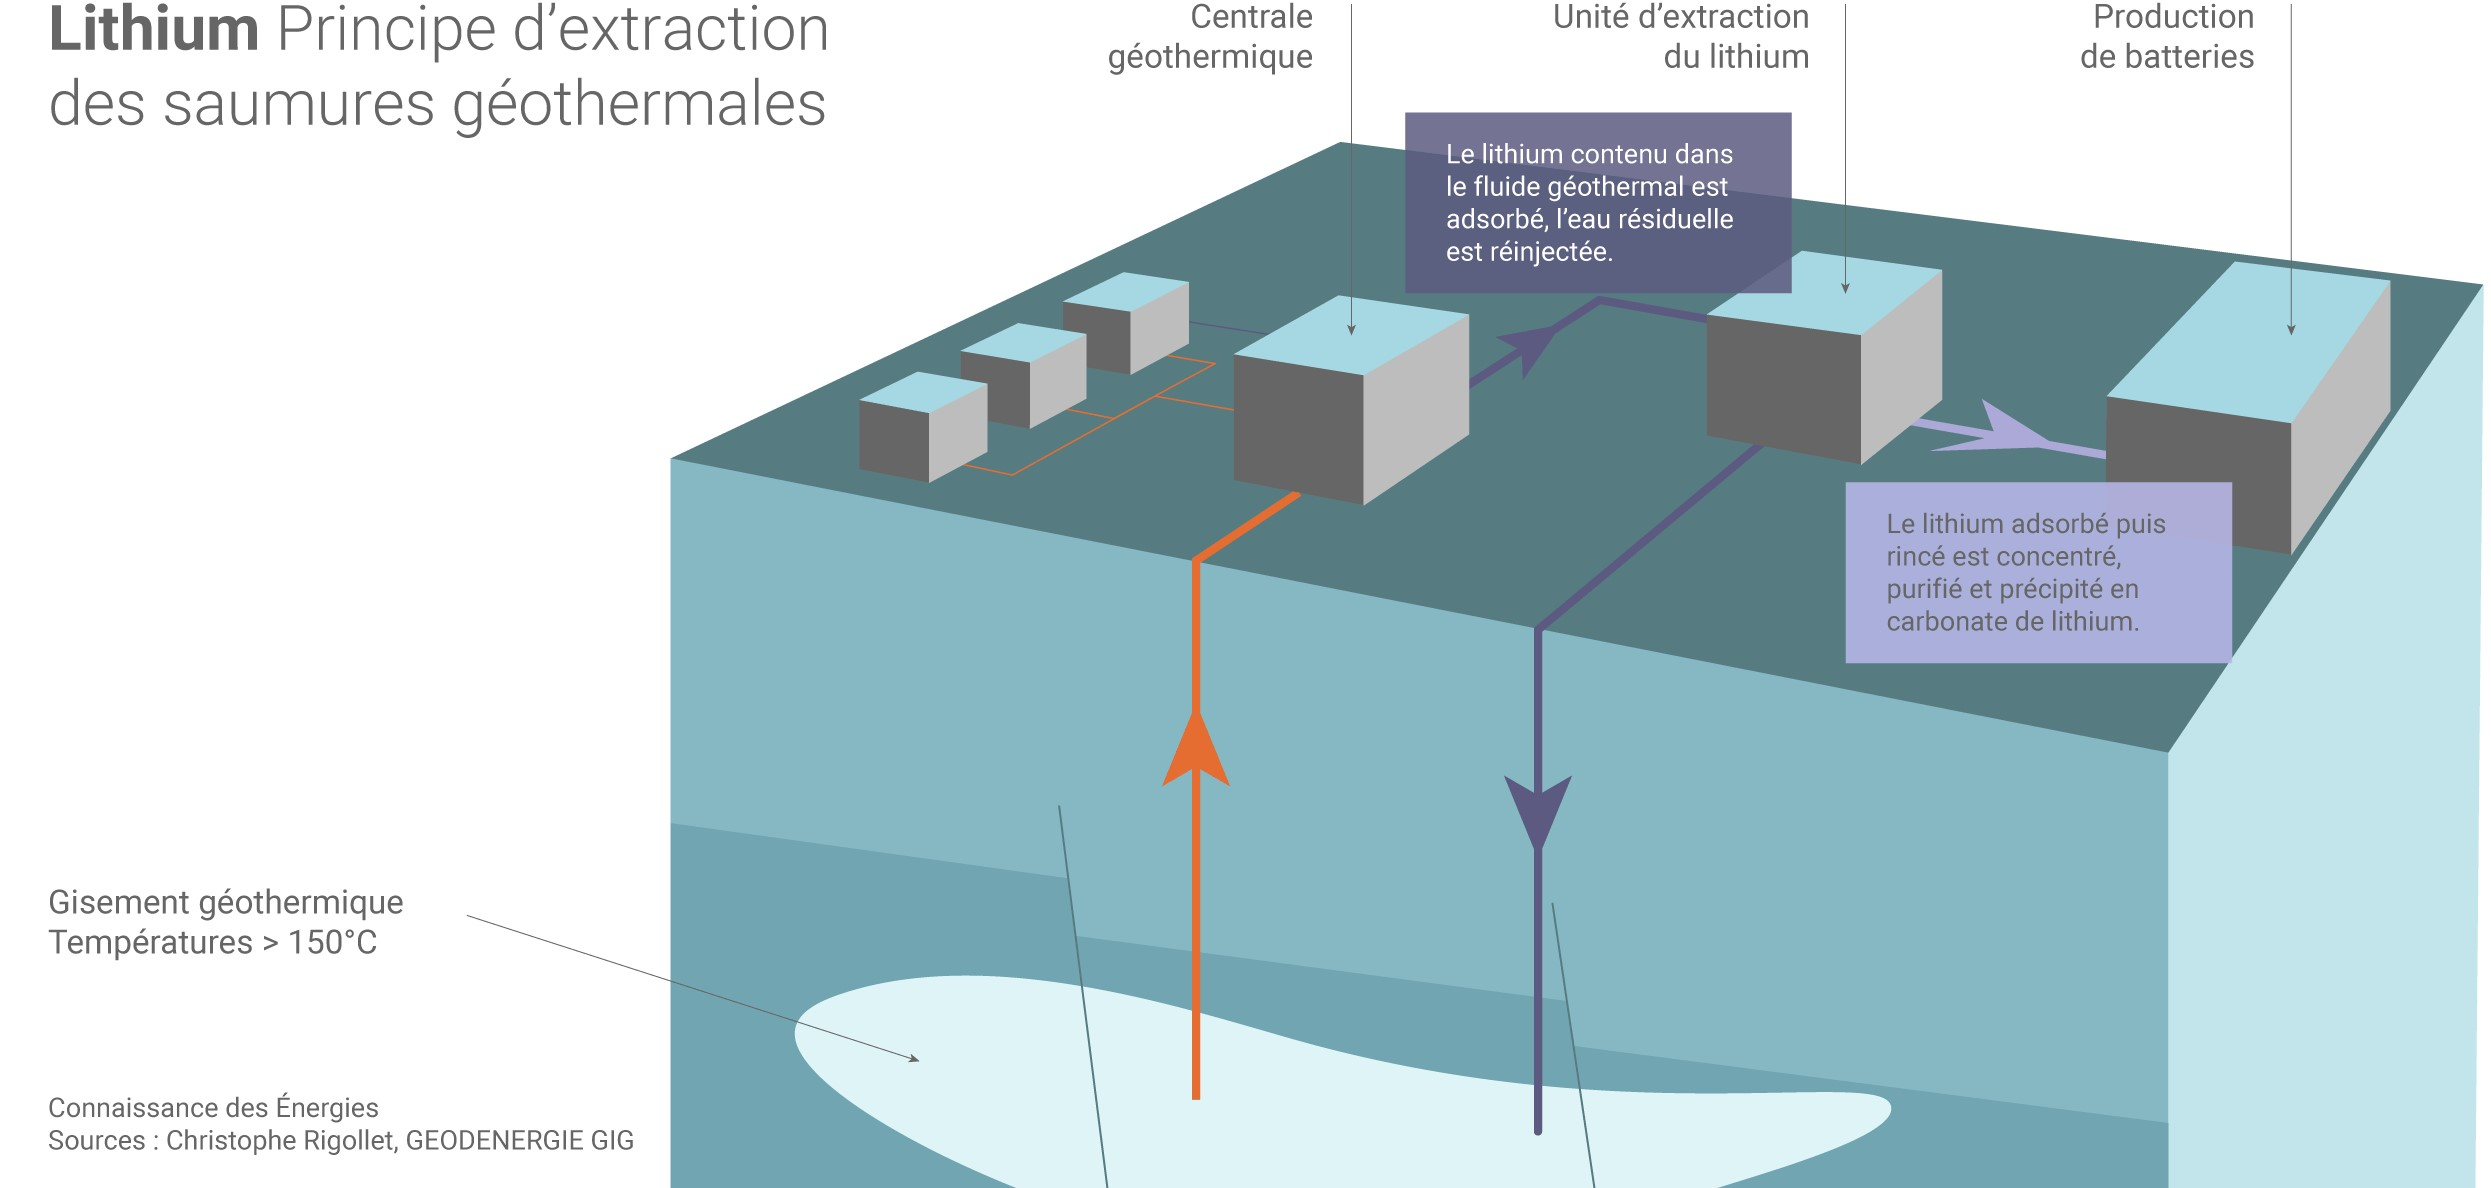
\includegraphics[width=0.65\textwidth]{Illustration métaux/extraction-lithium-geothermie-tribune-rigollet-tardieu-zoom.jpg}
  \end{center}
\end{wrapfigure}
\begin{center}
    \textbf{Opportunités}
\end{center}

L'approvisionnement en lithium comporte peu de risques spécifiques au-delà du stress hydrique sur l'approvisionnement. Des opportunités de production sont présentes en Union européenne. En Alsace, la coproduction possible de lithium est évalué à 15 000 tonnes par an sur 10 sites géothermique grâce à l'extraction du lithium des saumures. Le principe de l'extraction consiste à récupérer des eaux chaudes et riches en lithium entre 1000 et 4000 m de profondeur, d'en extraire la chaleur pour des usages énergétique et le lithium pour la production de batteries avant de remettre l'eau dans le sol.

% \begin{center}
%     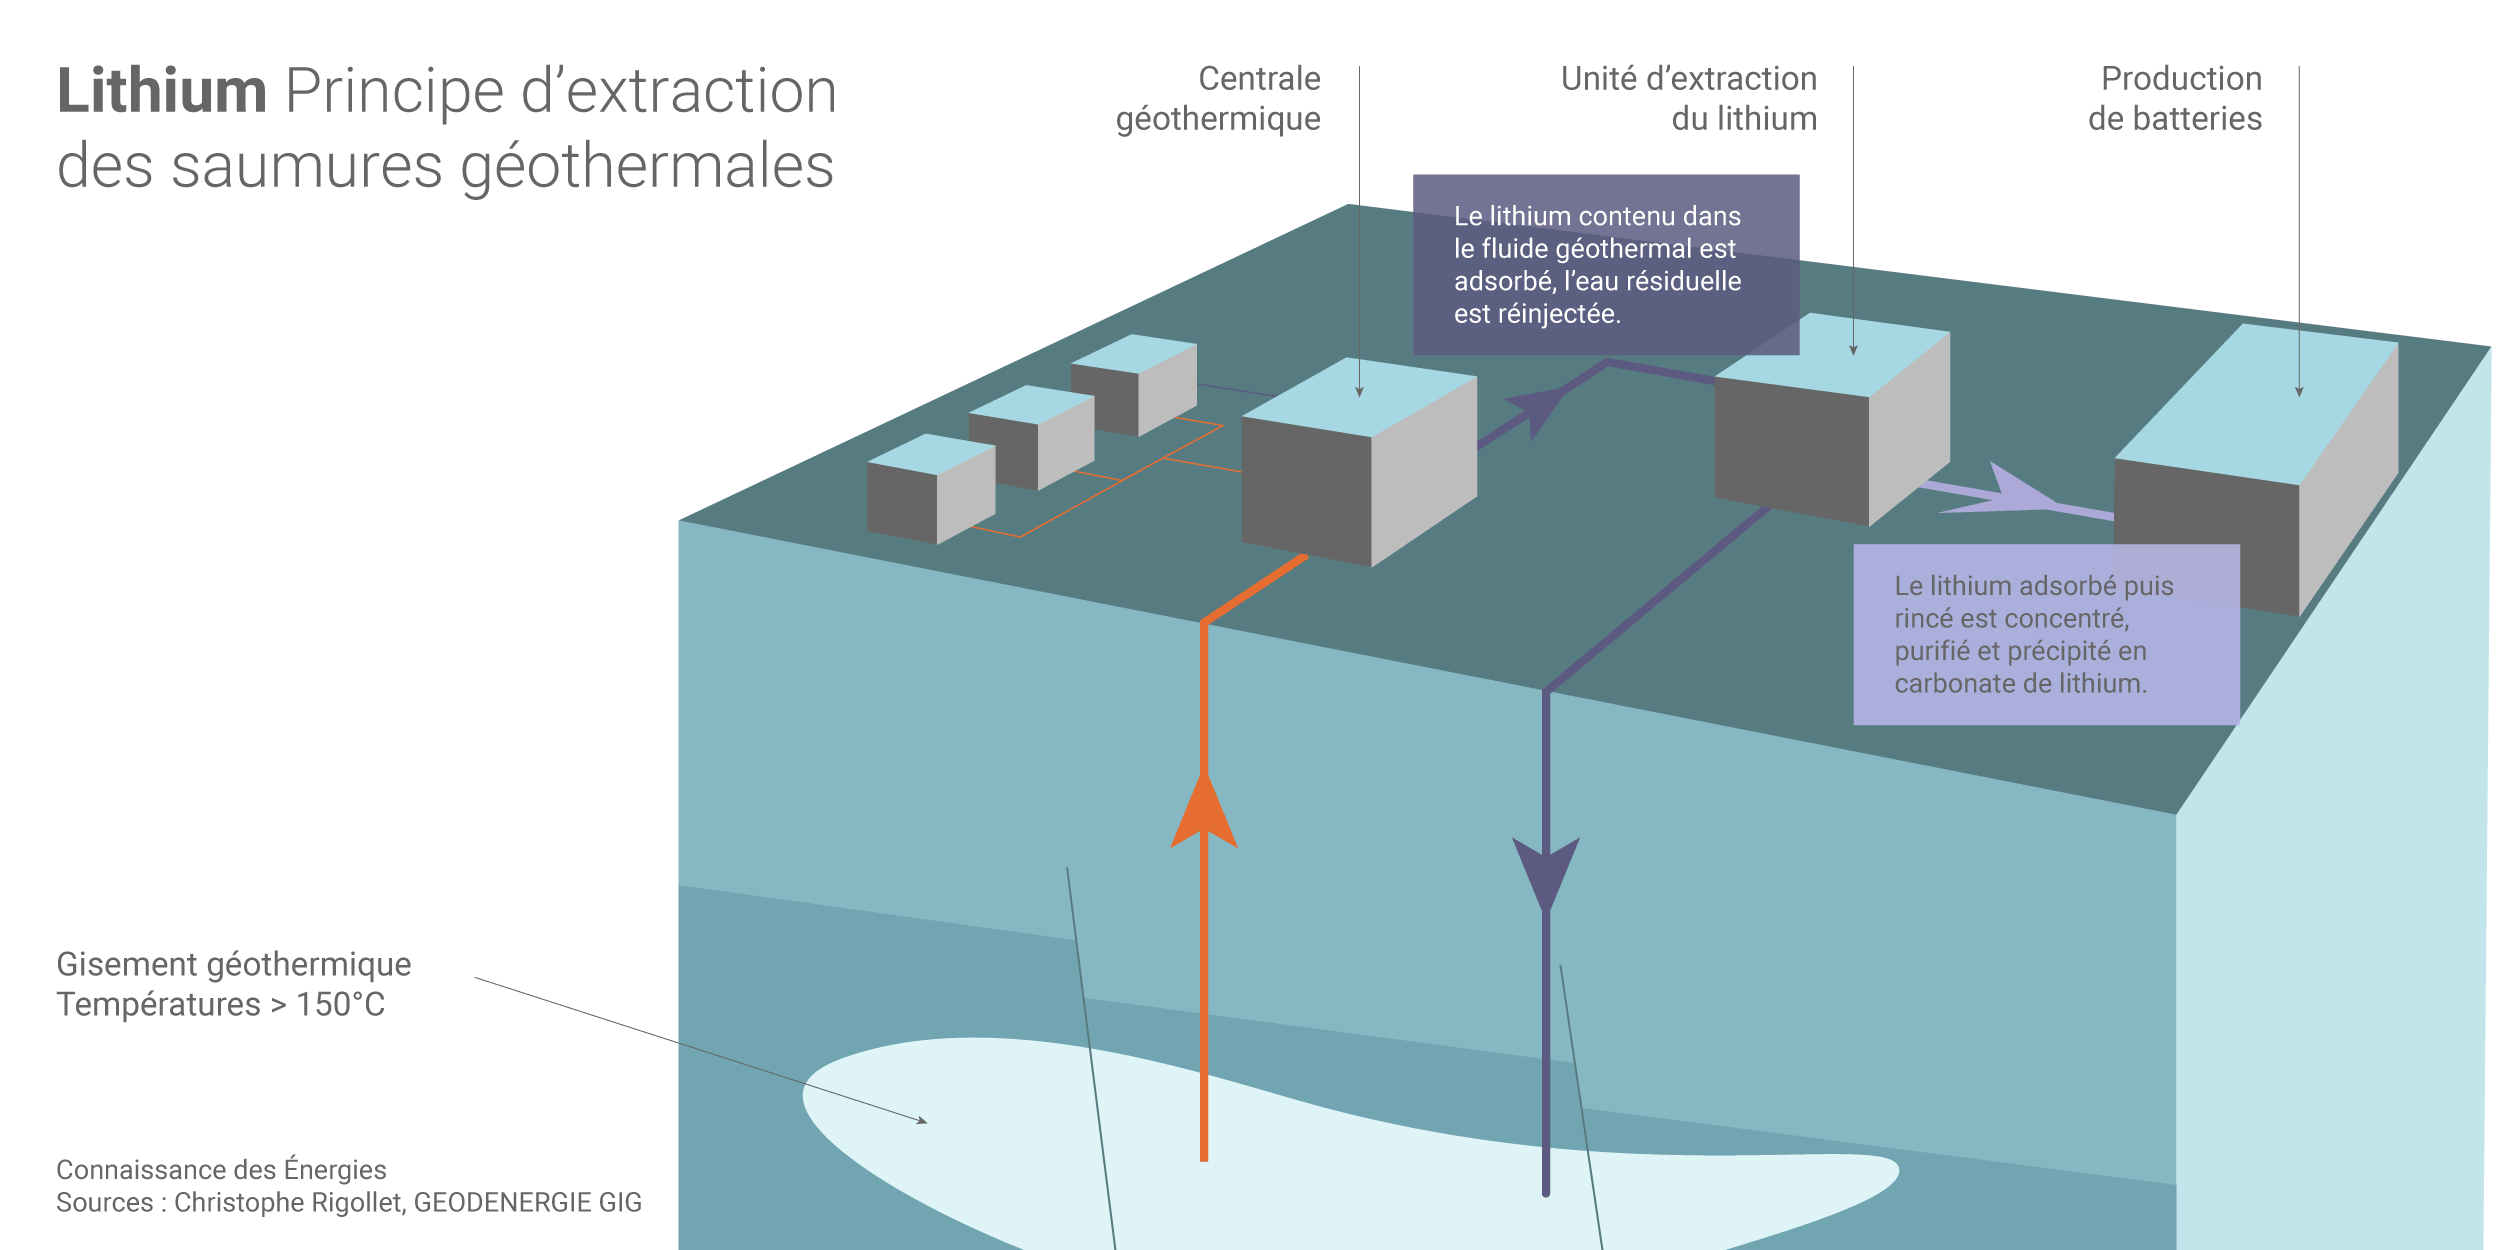
\includegraphics[width=10cm]{Illustration métaux/extraction-lithium-geothermie-tribune-rigollet-tardieu-zoom.png}
% \end{center}
